% Dies ist Teil der Vorlesung Physik auf dem Computer, SS 2012,
% Axel Arnold, Universitaet Stuttgart.
% 
% Dieses Werk ist unter einer Creative Commons-Lizenz vom Typ
% Namensnennung-Weitergabe unter gleichen Bedingungen 3.0 Deutschland
% zugänglich. Um eine Kopie dieser Lizenz einzusehen, konsultieren Sie
% http://creativecommons.org/licenses/by-sa/3.0/de/ oder wenden Sie sich
% schriftlich an Creative Commons, 444 Castro Street, Suite 900, Mountain
% View, California, 94041, USA.

\chapter{Einleitung}

In dieser Vorlesung geht es darum, wie der Computer in der modernen
Physik eingesetzt wird, um neue Erkenntnisse zu gewinnen. Klassisch
war die Physik ein Zusammenspiel aus Experiment und Theorie. Die
Theorie macht Vorhersagen, die im Experiment überprüft
werden. Umgekehrt kann im Experiment ein neuer Effekt beobachtet
werden, für den die Theorie eine Erklärung liefert. Durch den Einsatz
von Computern ist dieses Bild komplizierter geworden. In der folgenden
Graphik sind die Bereiche farblich hinterlegt, in denen heutzutage
Computer zum Einsatz kommen, die hellroten Bereiche werden in dieser
Vorlesung behandelt:
\begin{center}
  \tikzset{>=stealth',
    master/.style={rectangle,very thick,
      rounded corners,draw=black,font={\sffamily\bfseries\Large},
      node distance=6em and 0em},
    subnode/.style={rectangle,very thick,
      draw=black,fill=gray!10!white,font={\sffamily},
      node distance=0.2em},
    edge/.style={very thick},
    vorl/.style={fill=red!20!white}
  }
  \begin{tikzpicture}
    \node[master,vorl] (sim) {Simulation};
    \node[master,above left= of sim] (theo) {Theorie};
    \node[master,above right= of sim] (exp) {Experiment};
    \node[subnode,above left= of theo] (sym) {Symbolische Mathematik};
    \node[subnode,vorl,below left= of theo] (num) {Numerische Lösung};
    \node[subnode,above right= of exp] (ausw) {Steuerung};
    \node[subnode,vorl,below right= of exp] (mess) {Auswertung};

    \draw[edge] (theo) -- (sym);
    \draw[edge] (theo) -- (num);
    \draw[edge] (exp)  -- (ausw);
    \draw[edge] (exp)  -- (mess);

    \draw[edge,->] (theo) to [bend left] node[above] {Vorhersage} (exp);
    \draw[edge,->] (exp) to [bend left] node[below] {Überprüfung} (theo);

    \draw[edge,->] (exp.south) to [bend left=30] node[left] {Eichung} (sim.east);
    \draw[edge,->] (sim.east) to [bend right=60] node[right] {Vorhersage} (exp.south);

    \draw[edge,->] (theo.south) to [bend right=30] node[right] {Vorhersage} (sim.west);
    \draw[edge,->] (sim.west) to [bend left=60] node[left] {Überprüfung} (theo.south);
  \end{tikzpicture}
\end{center}
Zu den klassischen Säulen Theorie und Experiment ist die
\emph{Simulation} als Mittelding zwischen Theorie und Experiment
gekommen. Computersimulationen stellen Experimente im Computer nach,
ausgehend von bekannten theoretischen Grundlagen. Alles, für das es
Wechselwirkungstheorien gibt, kann simuliert werden, von Galaxien bis
hin zu Elektronen und Quarks. Dazu gibt es eine Vielzahl an
unterschiedlichen Methoden, deren Grundlagen in dieser Vorlesung
vorgestellt werden.

Simulationen erfüllen zwei Hauptaufgaben: Simulationen können
einerseits genutzt werden, um Experimente möglichst genau zu
reproduzieren, andererseits kann man auch abstrakte theoretische
Modelle in ihrer vollen Komplexität untersuchen.

Simulationen, die an ein Experiment angepasst (geeicht) sind, können
zusätzliche Informationen liefern, die experimentell nicht zugänglich
sind. Zum Beispiel kann man dort Energiebeiträge getrennt messen oder
sehr kurzlebige Zwischenprodukte beobachten. Außerdem erlauben
Simulationen, Wechselwirkungen und andere Parameter gezielt zu
verändern, und damit Vorhersagen über zukünftige Experimente zu
machen.

Simulationen, die auf theoretischen Modellen basieren, sind oft ein
gutes Mittel, um notwendige Näherungen auf Plausibilität zu überprüfen
oder um einen ersten Eindruck vom Verhalten dieses Modells zu
erhalten. Damit können Simulationen auch helfen, zu entscheiden, ob
notwendige Näherungen oder das Modell unvollständig ist, wenn Theorie
und Experiment nicht zu einander passen. Schließlich lassen sich,
anders als im Experiment, Wechselwirkungen einfach ausschalten, um
deren Einfluss abschätzen zu können.

In der klassischen theoretischen Physik werden Papier und Bleistift
zunehmend vom Computer verdrängt, denn \emph{Computeralgebra} ist
mittlerweile sehr leistungsfähig und kann zum Beispiel in wenigen
Sekunden komplexe Integrale analytisch lösen. Und falls eine Gleichung
doch einmal zu kompliziert ist für eine analytische Lösung, so kann
der Computer mit \emph{numerischen Verfahren} oft sehr gute Näherungen
finden. Letztlich passiert dies auch in einer Computersimulation,
allerdings hat sich dieses Feld soweit entwickelt, dass es mit Recht
als eigenständig bezeichnet wird.

In der experimentellen Physik fallen immer größere Datenmengen an. Der
LHC erzeugt zum Beispiel pro Jahr etwa 10 Petabyte an Daten, also etwa
200 Millionen DVDs, was über mehrere Rechenzentren verteilt
gespeichert und ausgewertet werden muss. Klar ist, dass nur Computer
diese gigantischen Datenmengen durchforsten können. Aber auch bei
einfacheren Experimenten helfen Computer bei der \emph{Auswertung und
  Aufbereitung} der Daten, zum Beispiel durch Filtern oder
statistische Analysen. Viele Experimente, nicht nur der LHC, sind aber
auch so komplex, dass Computer zur \emph{Steuerung} der Experimente
benötigt werden, was wir in dieser Vorlesung aber nicht behandeln
können. Die Auswertung und Aufbereitung der Daten hingegen wird
besprochen, auch weil dies genauso auch für Computersimulationen
benutzt wird.

Neben diesen direkten Anwendungen in der Physik ist der Computer
mittlerweile natürlich auch ein wichtiges Mittel für den
Wissensaustausch unter Physikern, sei es beim Schreiben
wissenschaftlicher Arbeiten oder beim internationalen Austausch über
E-mail und Videokonferenz. Auch stehen mittlerweile die meisten
wissenschaftlichen Arbeiten weltweit in elektronischen Bibliotheken
zur Verfügung. Leider hat das einfachere Publizieren mit Hilfe des
Computers auch zu einem starken Anstieg immer spezialisierter Arbeiten
geführt, so dass man zur Recherche in diesen riesigen Datenmengen
mittlerweile ebenfalls Computer benötigt.

Um den Computer für Simulationen, Auswertung von Daten oder auch
Lösung komplexer Differenzialgleichungen nutzen zu können, sind neben
physikalischen Kenntnissen auch solche in Programmierung, numerischer
Mathematik und Informatik gefragt. In diesem Skript geht es vor allem
um die grundlegenden Methoden und wie diese angewandt werden, daher
dominiert die numerische Mathematik etwas. Anders als in einer
richtigen Vorlesung zur Numerik stehen hier aber die Methoden und
Anwendungen anstatt der Herleitungen im Vordergrund.

\section{Über dieses Skript}

Im Folgenden wird eine in der numerischen Mathematik übliche Notation
benutzt. Wie auch in den meisten Programmiersprachen werden skalare
und vektorielle Variablen nicht durch ihre Schreibweise unterschieden,
allerdings werden üblicherweise die Namen $i$--$l$ für (ganzzahlige)
Schleifenindizes benutzt, $n$ und $m$ für Dimensionen. Da Schleifen sehr
häufig auftreten, wird hierfür die Kurznotation Anfang(Inkrement)Ende
benutzt. Zum Beispiel bedeuten
\begin{align*}
  1(1)n\,=\,1,2,\ldots, n\\
  n(-2)1\,=\,n, n-2,\ldots, 3, 1.
\end{align*}
Alle anderen Variablen sind reellwertige Skalare oder Vektoren,
$\RR^n$ bezeichnet dabei den $n$-dimensionalen Vektorraum reller
Zahlen. Mit $e_i$ wird dabei der Einheitsvektor der $i$-ten Spalte
bezeichnet, mit $e_i^T$ seine Transponierte, also der Einheitsvektor
der $i$-ten Zeile. Bei komplexen Vektoren steht entsprechend der obere
Index $^H$ für die Hermitesche eines Vektors, also die Transponierte
des Vektors, bei der alle Komponenten komplex konjugiert sind. Für
reelle Vektoren sind also $^H$ und $^T$ gleichbedeutend.

Integrale werden mit dem Volumenelement am Ende geschrieben, dessen
Dimensionalität sich aus dem Integrationsbereich erschließt. Sehr
häufig werden Abschätzungen mit Hilfe der \emph{Landau}-Symbole
verkürzt. Wie üblich heißt für zwei Funktionen $f$ und $g$
\begin{equation*}
  f = \O_{x\to a}(g) \quad\iff\quad \lim_{x\to a}
  \frac{\lvert f(x)\rvert}{\lvert g(x)\rvert}<\infty.
\end{equation*}
In den meisten Fällen ist $a=0$ oder $a=\infty$ und aus dem Kontext
klar, welcher Grenzwert gemeint ist. Dann wird die Angabe
weggelassen. Oft wird auch die Notation $f = g + \O(h)$ benutzt, um $f
+ g = \O(h)$ auszudrücken. $f(x) \dot{=} g(x)$ schließlich bedeutet,
dass $f$ und $g$ um Null herum in linearer Ordnung gleich sind, also
$f(x) - g(x) = \O_{x\to 0}(x)$.

Numerische Algorithmen werden in diesem Skript in der Sprache Python
\footnote{\url{http://python.org}} dargestellt. Dabei werden die
leistungsfähigen numerischen Erweiterungen NumPy und
SciPy\footnote{\url{http://www.scipy.org}} intensiv eingesetzt, und
zur Visualisierung dient die hervorragende matplotlib
\footnote{\url{http://matplotlib.org}}. Alle Graphen in dieser
Vorlesung sind mit matplotlib erstellt worden. Zum Erlernen von Python
sei auf die Materialien der Veranstaltung „Computergrundlagen“
verwiesen, die im Fachbereich Physik der Universität Stuttgart
jährlich angeboten wird.

Im Bereich des Hochleistungsrechnens werden vor allem die Sprachen
Fortran und C/C++ eingesetzt, weil diese in Verbindung mit guten
Compilern sehr effizienten Code ergeben. Allerdings verlangen diese
Sprachen die explizite Typisierung von Variablen, was Beispiele
unnötig verkompliziert. Zudem sind Speicherzugriffe nur ungenügend
geschützt, was die Fehlersuche sehr erschwert. Daher werden in dieser
Vorlesung und den zugehörigen Übungen C/C++ nicht eingesetzt.

Die meisten der in diesem Skript vorgestellten numerischen Methoden
werden von SciPy direkt unterstützt. Die Qualität dieser
Implementationen ist mit eigenem Code nur schwierig zu überbieten. Wo
immer möglich, wird daher auf die entsprechend SciPy-Befehle
verwiesen. Zum Beispiel wird auf die Funktion "`method"' im
SciPy-Modul "`library"' in der Form
\scipy{scipy.library.method(arg1, arg2,...)} verwiesen. Trotzdem
sind viele Methoden auch als expliziter Code gezeigt, da man natürlich
eine Vorstellung davon haben sollte, was diese Methoden tun.

\section{Beispiel: Fadenpendel}
\index{Fadenpendel}

\begin{figure}
  \centering
  \newcommand{\auslenkung}{50}
  \newcommand{\kraft}{1.5}
  \begin{tikzpicture}[x=3em,y=3em]
    \draw[dashed] (0,1)--(0,-2.5);

    % Winkel
    \filldraw[fill=none,draw=black] (0,-1.5) arc (-90:-90-\auslenkung:1.5);
    \pgftransformrotate{-\auslenkung/2}
    \node at (-0.0,-1) {$\alpha$};
    \pgftransformrotate{\auslenkung/2}

    % ausgelenkte Kugel
    \pgftransformrotate{-\auslenkung}

    \draw[color=black,dashed] (0,1) -- (0,-3);
    \draw[thick,fill] (0,-3) circle (0.18cm) node (masse) {};
    \draw[thick] (0,0) circle (.1cm);
    \draw[thick] (0,0) -- (0,-3);
    \draw[decorate,decoration=brace] (-.2,-3) -- (-.2,0);
    \node at (-0.7,-1.5) {$l$};

    \draw[->,color=blue,thick] (masse) -- +({\kraft*sin(\auslenkung)},0)
    node (ft) {} node[right] {$F_\text{tan} = F_\text{G}\sin(\alpha)$};
    \draw[->,color=red,thick] (masse) -- +(0,{-\kraft*cos(\auslenkung)})
    node (fr) {} node[left] {$F_\text{rad}$};

    % totale Kraft
    \pgftransformrotate{\auslenkung}
    \draw[->,very thick] (masse) -- +(0,-\kraft)
    node (fg) {} node[below] {$F_\text{G} = -mg$};
    \draw[thin,dotted] (fr.center) -- (fg.center) -- (ft.center);
  \end{tikzpicture}
  \caption{Schematisches Fadenpendel der Masse $m$, das an einem
    masselosen, steifen Faden der Länge $l$ hängt.}
  \label{fig:pendel}
\end{figure}

Wir betrachten ein einfaches Beispielsystem, nämlich ein Fadenpendel.
Wird dieses Pendel nun ausgelenkt, vollführt es eine periodische
Schwingung um die Ruhelage, \dh\,, den tiefsten Punkt. Unser Ziel als
Physiker ist nun, die Position der Kugel als Funktion der Zeit
vorherzusagen. Das allerdings ist eine unmögliche Aufgabe --- man
stelle sich zum Beispiel eine stark inhomogene Masse vor (oder ein
Fadenpendel als Masse) oder dass der Faden elastisch ist. Daher müssen
wir zunächst ein geeignet vereinfachtes \emph{Modell} erstellen, auf
das wir dann die bekannten physikalischen Gesetze anwenden
können.

\subsection{Modell}

Als Modell wählen wir eine homogene Kugel der Masse $m$, die an einem
masselosen, steifen Faden der Länge $l$ hängt (vergleiche
Figur~\ref{fig:pendel}). Auf diese Kugel wirkt nur eine Gewichtskraft
der Größe $mg$ senkrecht nach unten, alle anderen Kräfte vernachlässigen wir
komplett, insbesondere auch die Reibung.

Da der Faden unendlich steif sein soll, kann sich die Kugel lediglich auf
einem Kreis mit Radius $l$ um die Aufhängung bewegen, \dh die
Position der Kugel ist durch die Auslenkung $\alpha$ aus dem tiefsten
Punkt vollständig beschrieben. Weiter wird die Komponente der Kraft
parallel zum Faden komplett von diesem kompensiert, daher bleibt bei
Auslenkung $\alpha$ von der Gewichtskraft nur ihre Komponente
\begin{equation}
  F_\text{tan} = F_\text{G}\sin(\alpha) = -mg\sin(\alpha)
\end{equation}
senkrecht zum Faden übrig. Das Newtonsche Gesetz besagt nun, dass
die Tangentialbeschleunigung, also die Beschleunigung entlang $\alpha$
\begin{equation}
  l\ddot\alpha = F_\text{tan}/m = -g\sin(\alpha)
  \label{eq:pendelgln}
\end{equation}
beträgt. Dies ist jetzt eine Differentialgleichung für die Auslenkung
$\alpha(t)$ des Pendels als Funktion der Zeit. Diese wiederum liefert
uns die gewünschte Position $(\cos(\alpha)l,\sin(\alpha)l)$ der Kugel
relativ zur Aufhängung als Funktion der Zeit. Leider hat selbst diese
einfache Differentialgleichung keine geschlossene Lösung, und wir
müssen weitere Näherungen einführen, um eine geschlossene analytische
Lösung zu erhalten.

\subsection{Näherung: der harmonische Oszillator}

\begin{figure}
  \centering
  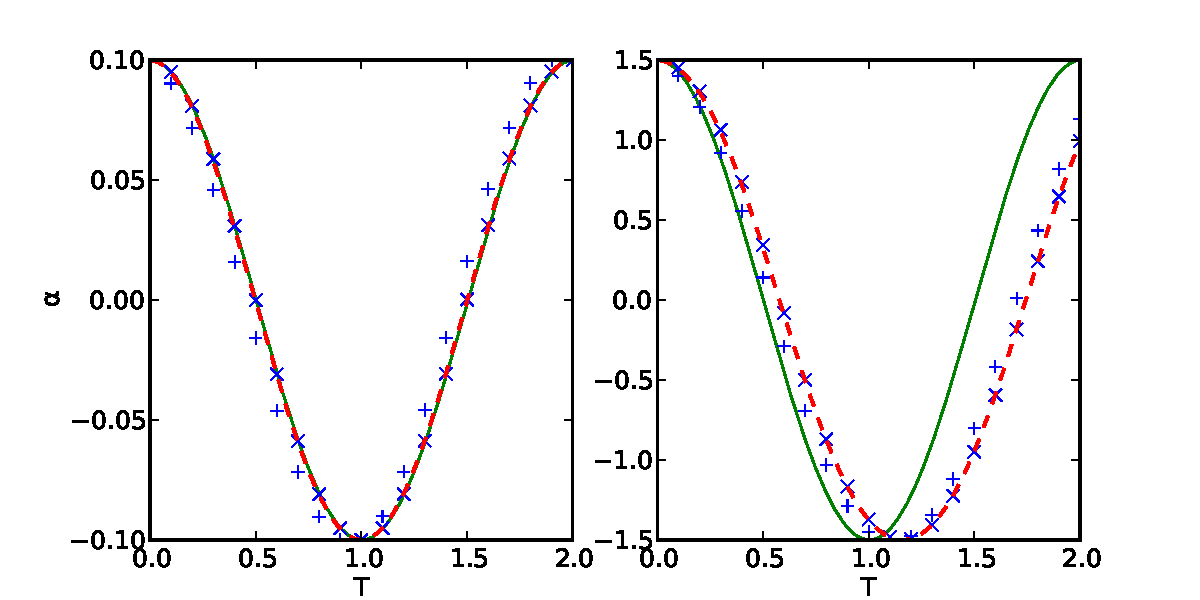
\includegraphics[width=\textwidth]{plots/pendel_loesung}
  \caption{Lösungen für ein Fadenpendel der Länge $l=1m$. Im linken
    Graphen ist die Ausgangslage $\alpha=1,5$, im rechten
    $\alpha=0,1$; in beiden Fällen ist die Ausgangsgeschwindigkeit
    0. Die durchgezogene grüne Linie markiert die analytische
    Näherungslösung \eqref{eq:naeherung} für kleine Winkel. Blaue $+$
    markieren die Schritte einer Integration mit dem einfachen
    Vorwärtsschrittverfahren \eqref{eq:simple} mit Zeitschritt $0,1s$,
    die gestrichelte rote Linie mit Zeitschritt $0,01s$. Blaue
    $\times$ markieren die Lösung mit Hilfe des
    Velocity-Verlet-Algorithmus und Zeitschritt $0,1s$.}
  \label{fig:loesung}
\end{figure}

Für kleine Winkel gilt $\sin(\alpha)\approx\alpha$, und damit
\begin{equation}
  \label{eq:harmosz}
  \ddot\alpha \approx -\frac{g}{l}\alpha.
\end{equation}
Diese Differentialgleichung beschreibt einen harmonischen Oszillator
mit Eigenfrequenz $\omega=\sqrt{g/l}$ und hat die allgemeine Lösung
\begin{equation}
  \alpha(t) = A cos(\omega t) + B sin(\omega t)
  \label{eq:naeherung}
\end{equation}
wie man leicht durch Einsetzen überprüft. Die Größen $A$ und $B$
ergeben sich aus den Anfangsbedingungen, nämlich der Anfangsposition
\begin{align}
  \alpha(0) = A \cos(0) + B \sin(0)
  &\quad\implies\quad A= \alpha(0)
\intertext{und "~geschwindigkeit}
  \dot\alpha(0) = -A \omega \sin(0) + B \omega \cos(0)
  &\quad\implies\quad B= \dot\alpha(0)/\omega.
\end{align}
Wir haben nun eine geschlossene Lösung für die Position des Pendels,
sofern die Ausgangslage nicht zu sehr ausgelenkt und die
Ausgangsgeschwindigkeit nicht sehr hoch ist. Ist das nicht der Fall,
erreicht die Lösung $\alpha(t)$ Werte, bei denen die Näherung
$\sin(\alpha)\approx \alpha$ stark verletzt ist. Die Lösung ist also
nicht \emph{konsistent} mit unserer vereinfachenden Annahme und daher
physikalisch sinnlos. Um diese Lösung zu visualisieren, nutzt man
heute üblicherweise den Computer, siehe Graph~\ref{fig:loesung}.

\subsection{Numerische Lösung}

Was passiert nun, wenn das System stärker ausgelenkt ist? Mit sehr
viel mehr Aufwand lässt sich auch für diesen Fall eine analytische,
allerdings nicht geschlossene Lösung in Form einer unendlichen Reihe
finden. Eine Alternative ist, die Differentialgleichung
\eqref{eq:pendelgln} mit Hilfe des Computers zu lösen. Wir sagen, wir
"`simulieren"' das Pendel. Dazu fixieren wir ein Einheitensystem, zum
Beispiel eine Sekunde als Zeiteinheit und einen Meter als
Längeneinheit. Wir betrachten ein einen Meter langes Pendel, daher ist
$l=1$, $g\approx 9,81$ und $\omega\approx 3,13$.

Diese Wahl des Einheitensystems kommt nicht von ungefähr. Natürlich
hätten wir genauso gut die Länge in Nanometern und die Zeit in Stunden
messen können. Dann wäre allerdings $l=10^9$, $g\approx 1,27\cdot
10^{17}$ und $\omega\approx 11.270$. Damit lässt sich zwar im Prinzip
genausogut rechnen, allerdings ist es meist besser, das
Einheitensystem so zu wählen, dass alle wesentlichen Größen nicht um
mehr als ein bis zwei Größenordnungen von ein abweichen. Denn wenn wir
dann in unserer Simulation eine Winkelgeschwindigkeit von $10^{30}$
oder mehr beobachten, können wir ziemlich sicher sein, dass unser
Programm noch fehlerhaft ist. Daher werden zum Beispiel molekulare
Simulationen üblicherweise nicht in SI-Einheiten formuliert, sondern
in Nanometern und Femtosekunden --- nicht anders, als auch die
Ergebnisse üblicherweise berichtet werden.

Zunächst müssen wir das Problem aber für den Computer anpassen, der ja
nur mit (endlich vielen) Zahlen rechnen kann, wir müssen das Problem
\emph{diskretisieren}. Wir betrachten nur die Zeitpunkte
\begin{equation}
  t_n = n\delta t, n=0(1)N,
\end{equation}
wobei der Zeitschritt $\delta t$ frei wählbar ist. Je kleiner $\delta
t$, desto genauer können wir $\alpha(t)$ bestimmen, allerdings steigt
natürlich die Anzahl der Schritte, die nötig sind, um eine feste
Gesamtzeit zu erreichen. Unsere Lösung, die Funktion $\alpha(t)$ wird
also durch ihre Werte $\alpha(t_n)$ an den diskreten Zeitpunkten
dargestellt.

\begin{figure}
  \centering
  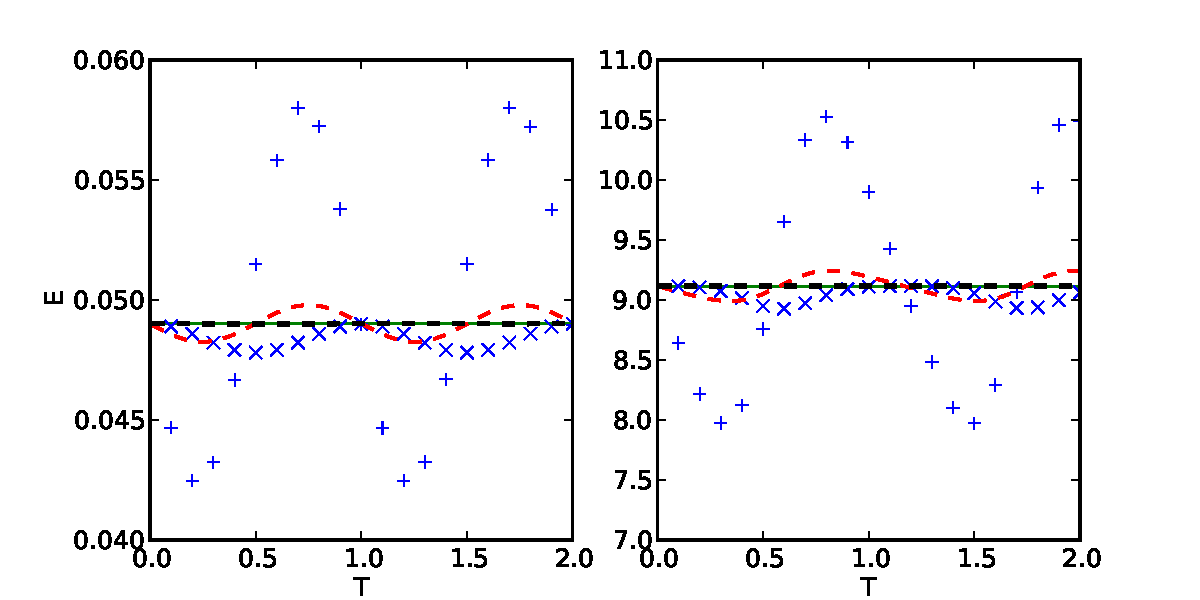
\includegraphics[width=\textwidth]{plots/pendel_energie}
  \caption{Energie als Funktion der Zeit, wieder für $l=1m$, und
    Ausgangslage $\alpha=1,5$ (links) und $\alpha=0,1$ (rechts) in
    Ruhe.  Blaue $+$ markieren die Ergebnisse einer Integration mit
    dem einfachen Vorwärtsschritt \eqref{eq:simple} mit Zeitschritt
    $0,1s$, die gestrichelte rote Linie mit Zeitschritt $0,01s$. Blaue
    $\times$ markieren die Lösung mit Hilfe des
    Velocity-Verlet-Algorithmus und Zeitschritt $0,1s$, und die
    gestrichelte schwarze Linie mit $0,01s$. Grün ist die erwartete
    Energie dargestellt, die nicht von der feinen Verlet-Integration
    zu unterscheiden ist.}
  \label{fig:energie}
\end{figure}

Um Gleichung \eqref{eq:pendelgln} auf den Computer zu bringen, müssen
wir uns allerdings noch überlegen, wie wir mit der Ableitung verfahren.
Da wir die Ausgangsposition und "~ge\-schwin\-dig\-keit gegeben haben, liegt
es nahe, die Gleichung zu integrieren:
\begin{equation}
  v(t+\delta t) = \dot\alpha(t + \delta t) = v(t) + \int_{t}^{t+\delta t}
  -\omega^2\sin \alpha(\tau)\, d\tau.
\end{equation}
Da $\delta t$ aber unser Zeitschritt ist, wir also nichts weiter über
$\alpha(\tau)$ wissen, bietet sich die folgende lineare Näherung an:
\begin{equation}
  v(t+\delta t) \approx v(t) - \omega^2\sin\alpha(t) \delta t.
\end{equation}
Analog ergibt sich dann durch nochmalige Integration:
\begin{equation}
  \alpha(t+\delta t) \approx \alpha(t) + v(t) \delta t.
  \label{eq:simple}
\end{equation}
Ausgehend von
\begin{equation}
  \alpha(0) = \alpha_0 \quad\text{und}\quad v(0) = v_0
\end{equation}
lässt sich damit also $\alpha(t)$ numerisch bestimmen. Der
Quellcode~\ref{lst:pendel} zeigt bei Wahl der "`simple"'-Methode, wie
eine einfache Implementation in Python aussehen könnte.

Wie kann man nun überprüfen, ob diese Lösung tatsächlich korrekt ist?
Da das System abgeschlossen ist, muss seine Energie
\begin{equation}
  E = \frac{1}{2} l^2 v(t)^2 + gl (1 - \cos \alpha(t))
\end{equation}
erhalten sein. Lässt man sich diese allerdings ausgeben, stellt man
fest, dass $E(t)$ erheblich schwankt, vergleiche
Graph~\ref{fig:energie}. Dies lässt sich durch Verringern des
Zeitschritts beheben, das kostet aber entsprechend mehr Rechenzeit.

Eine bessere Alternative ist, den Algorithmus zu verbessern, was
wiederum etwas analytische Arbeit erfordert. Wir werden im Laufe der
Vorlesung verstehen, wie mit Hilfe von Taylorentwicklungen ein
besseres Verfahren gefunden werden kann, der sogenannte
\emph{Velocity-Verlet-Algorithmus}:
\begin{align}
  v\left(t + \frac{\delta t}{2}\right) &= v(t) + \frac{\delta t}{2} F(t) \\
  \alpha(t + \delta t) &= \alpha(t) + \delta t\, v\left(t + \frac{\delta t}{2}\right) \\
  v(t + \delta t) &= v\left(t + \frac{\delta t}{2}\right) + \frac{\delta t}{2}
  F(t + \delta t),
\end{align}
der anders als die zuerst angegebene Vorgehensweise numerisch stabil
ist und quasi keine Energieschwankungen aufzeigt, vergleiche
Graph~\ref{fig:energie}.  Interessant ist, dass formal die
Geschwindigkeiten zu halben Zeitschritten eingehen. Im
Quellcode~\ref{lst:pendel} ist alternativ auch dieser Integrator
implementiert. Obwohl er nur unwesentlich komplizierter ist als der
einfache Integrator zuvor, erreicht etwa dieselbe Genauigkeit wie
dieser mit einem Zehntel der Zeitschritte.

Als weiterer Test bietet sich an, bei kleinen Auslenkungen mit der
analytisch bekannten Lösung zu vergleichen, die gut reproduziert wird,
siehe Graph~\ref{fig:loesung}. Bei größeren Anfangsauslenkungen oder
-ge\-schwin\-dig\-keiten ist die Abweichung allerdings sehr groß, weil
hier die analytische Näherung versagt. Im Rahmen ihrer Genauigkeit
erlaubt also die numerische Lösung, das vorgegebene Modell in einem
größeren Parameterraum auf sein Verhalten hin zu untersuchen, als
analytisch möglich wäre.

\lstinputlisting[style=floating,firstline=10,
caption={[Fadenpendel] Python-Code zum Fadenpendel
  mit graphisch aufbereiteter Ausgabe mit Hilfe der \texttt{matplotlib}.},
label=lst:pendel]{pendel.py}

%%% Local Variables: 
%%% mode: latex
%%% TeX-master: "padc"
%%% TeX-PDF-mode: t
%%% End: 
